% This is LLNCS.DEM the demonstration file of
% the LaTeX macro package from Springer-Verlag
% for Lecture Notes in Computer Science,
% version 2.4 for LaTeX2e as of 16. April 2010
%

\documentclass{llncs}
\usepackage{epstopdf}
%
%\usepackage[dvips]{graphicx}
\usepackage{epsfig}
%\usepackage[chapter]{theorems}
\usepackage{symbols}
\usepackage{url}
\usepackage{algorithm}
\usepackage{algorithmic}
\usepackage{color}
\usepackage{alltt}
\usepackage{dsfont}
\usepackage{upgreek}
\usepackage[tight]{shorttoc}
\usepackage{multirow}
\usepackage{rotating}
\usepackage{array}
\usepackage{colortbl}
\usepackage{xcolor}
\usepackage{listings}
\usepackage[rounded]{syntax}
\usepackage{slashbox}
\usepackage{graphicx, subfig}
\usepackage{enumerate}
\usepackage{amssymb}
\usepackage{appendix}
\usepackage{eurosym}
\usepackage{amsfonts}
\usepackage{pifont}
%\usepackage{hyperref}
\usepackage{pdflscape}
\usepackage{amsmath}
\usepackage{fixltx2e} 

\lstset{ %
        language=Prolog,                % the language of the code
        basicstyle=\scriptsize,       % the size of the fonts that are used for the code
        numbers=right,                   % where to put the line-numbers
        numberstyle=\scriptsize,      % the size of the fonts that are used for the line-numbers
        stepnumber=1,                   % the step between two line-numbers. If it's 1, each line 
                                % will be numbered
        numbersep=0.05cm,                  % how far the line-numbers are from the code
        backgroundcolor=\color{white},  % choose the background color. You must add \usepackage{color}
        showspaces=false,               % show spaces adding particular underscores
        showstringspaces=false,         % underline spaces within strings
        showtabs=false,                 % show tabs within strings adding particular underscores
        frame=none,                   % adds a frame around the code
        tabsize=3,                      % sets default tabsize to 2 spaces
        captionpos=b,                   % sets the caption-position to bottom
        breaklines=true,                % sets automatic line breaking
        breakatwhitespace=false,        % sets if automatic breaks should only happen at whitespace
        %title=\lstname,                 % show the filename of files included with \lstinputlisting;
                                   % also try caption instead of title
        escapeinside={\%*}{*)},         % if you want to add a comment within your code
        deletekeywords={not}
        %morekeywords={luents, actions, always, initial, if, inertial, after, inertial, noConcurrency,goal,not,caused,executable,nonexecutable,forbiden,requires}            % if you want to add more keywords to the set
}
\newcommand{\hlight}[2]{\begingroup \color{#1}#2 \endgroup}
\newcommand{\manolo}[2]{{\hlight{#1}{#2}}}

\def\ie{\textit{i.e.}}
\def\eg{\textit{e.g.}}
\def\cf{\textit{cf.}}
\def\aka{\textit{a.k.a.}}

\include{apis}
\newcommand\SeQLcode[3]{
	\lstinputlisting[language=SQL, morekeywords= {now, top}, caption={#1}, columns=fixed, label=#3]{#2}
}

\newcommand\PrologCode[3][]{
	\lstinputlisting[language=Prolog, morekeywords={fluents, actions, always, initial, if, inertial, after, inertial, noConcurrency,goal,not,caused,executable,nonexecutable,forbiden,requires}, caption={#1}, columns=fixed, label=#3]{#2}
}

\newcommand{\tickYes}{\checkmark}

\newcommand{\tickNo}{\hspace{1pt}\ding{55}}

\newcommand\dt[1]{$\mathtt{#1}$}

\newcommand{\sembrack}[1]{[\![#1]\!]}

\hyphenation{pro-du-cer ca-ta-log coor-di-na-tes de-pen-dent ge-ne-ra-tion pa-ra-lle-li-za-tion con-ti-nuous im-ple-men-ting exe-cu-tion apli-ca-tion acce-ssing answer know-ledge po-ssi-ble gene-rated abs-trac-tion diffe-rent}
\newcommand\tabsize[2]{
\begin{table}
   \begin{center}
       {\small
      \begin{tabular}{m{0.6cm} |m{1.4cm} m{1.4cm} m{1.4cm} m{1.4cm} }
  
         \hline
          \multirow{2}{*}{$l$}& \multicolumn{4}{c}{Workflows}\\
            & \textbf{W1} & \textbf{W2} & \textbf{W3} & \textbf{W4} \\
         \hline
         \hline
6 & 0 & 0 & 0 & 0 \\
7 & 4 & 4 & 20 & 20 \\
8 & 62 & 128 & 598 & 1192 \\
9 & 278 & 956 & 5062 & 15820 \\
10 & 578 & 3068 & 19822 & 90100 \\
11 & 718 & 5368 & 43698 & 277800 \\
12 & 718 & 6268 & 62358 & 525476 \\
13 & 718 & 6268 & 62358 & 749840 \\
14 & 718 & 6268 & 62358 & 749840 \\
         \hline     
      \end{tabular}
   }  
      \caption{#2}\label{#1}
      
     \end{center}
   \end{table}  
}

\newcommand\tabtime[2]{
\begin{table}
   \begin{center}
      \begin{tabular}{m{0.6cm} |m{1.4cm} m{1.4cm} m{1.4cm} m{1.4cm}}
         \hline
          \multirow{2}{*}{$l$}& \multicolumn{4}{c}{Workflows}\\
                              & \textbf{W1} & \textbf{W2} & \textbf{W3} & \textbf{W4} \\
         \hline
         \hline
 6&  0,00 & 0,00 & 0,00 & 0,00 \\
 7&  0,00 & 0,00 & 0,00 & 0,00 \\
 8&  0,00 & 0,00 & 0,01 & 0,02 \\
 9&  0,01 & 0,00 & 0,15 & 0,47 \\
 10&  0,07 & 0,00 & 2,30 & 8,13 \\
 11&  0,37 & 2,00 & 16,04 & 66,30 \\
 12&  2,34 & 11,00 & 81,24 & 312,18 \\
 13&  8,44 & 46,00 & 170,39 & 787,00 \\
         \hline
      \end{tabular}
      \caption{#2}\label{#1}
     \end{center}
   \end{table}
}

%
\begin{document}
%&&&&&&&&&&&&&&&

\title{A Service Composition Approach for Data-Centric Workflows}
%
\titlerunning{A Service Composition Approach for Data-Centric Workflows}  % abbreviated title (for running head)
%                                     also used for the TOC unless
%                                     \toctitle is used
%
\author{
Carlos-Manuel L\'opez-Enr\'iquez\inst{2} \and V\'ictor Cuevas-Vicentt\'in\inst{3} \and Genoveva Vargas-Solar\inst{1,2}
\and Christine Collet\inst{2} \and Jos\'e-Luis \\Zechinelli-Martini\inst{4}
}
%
\authorrunning{L\'opez-Enr\'iquez et al.} % abbreviated author list (for running head)
%
%%%% list of authors for the TOC (use if author list has to be modified)
\tocauthor{Carlos-Manuel L\'opez-Enr\'iquez, V\'ictor Cuevas-Vicentt\'in, Genoveva Vargas-Solar, Christine Collet, Jos\'e-Luis \\Zechinelli-Martini}
%
\institute{
CNRS \and Grenoble Institute of Technology\\ BP. 72, 38402, Saint Martin d'H\`{e}res Cedex, France\\
\and
University of California at Davis\\ One Shields Avenue, Davis CA 95616, USA\\ 
\and
Exhacienda Sta. Catarina M\'{a}rtir s/n 72820 \\ San Andr\'{e}s Cholula, Puebla, Mexico \\
\email{carlos.manuel.lopez@gmail.com},\email{victorcuevasv@gmail.com},\email{genoveva.vargas@gmail.com},\\
\email{christine.collet@grenoble-inp.fr},\email{joseluis.zechinelli@udlap.mx} 
}


\maketitle              % typeset the title of the contribution

\begin{abstract}

This paper presents our approach for specifying, transforming, and enacting data-centric workflows in a service-oriented environment. First, we propose ASASEL (Abstract State Machines Execution Language) a language and system based on the ASM formalism for specifying workflows consisting of on-demand and streaming data services that produce data, which are then processed by simple and composite computation services as well as by operations on complex values. Second, we present our initial characterization of a planning-based approach for the transformation of workflows. In particular, we address the exploration of parallelism through the workflow structure. Together, our language and enactment engine along with our transformation approach provide the foundation for a highly flexible mechanism for managing data-centric workflows, and which can also be adapted to other domains such as business processes or eScience.

\keywords{workflows, services, answer set planning, logic programming}
\end{abstract}
%

	
\section{Introduction}\label{sec:asasel:intro}

%The advances in mobile computing and communication bring promises of timely and inexpensive access to information, as well as of %increasing interaction between people and software agents. 
%Service-oriented architectures play a crucial role in these developments, since they  deal with the interoperability issues of the %underlying systems.

%We note in particular 
%This phenomenon is due to the 
We witness a proliferation of streaming and on-demand data services for accessing data pertaining to a multitude of domains, possibly involving temporal and mobile properties. The availability of data services is accompanied by a democratization in access to computational resources. Nevertheless, users typically must rely on proprietary applications that delegate data processing to their backend, which makes it difficult to share resources and add new features.	
	
Therefore we propose ASASEL (Abstract State Machines Execution Language) to build up systems from shared resources accessible as services via data-centric workflow specifications. Our work considers both on-demand and streaming data services producing complex values, operations on these data, and the ability to construct composite computation services to process them. In addition, we propose a workflow transformation framework 
%currently under development 
based on planning techniques to meet quality of service goals. We present a concrete implementation of this framework covering parallelization through the workflow structure.

The remainder of this paper is structured as follows. Section \ref{sec:dataCentricWorkflows} presents our workflow model and language, while Section \ref{sec:complexValuesDataModel} introduces our complex values data model and related operations. In Section \ref{sec:workflowTransformation} we present a planning-based workflow transformation framework, whose experimental results are presented in Section \ref{sec:experiments}. Our system implementation is discussed in Section \ref{sec:systemImplementation}. Section \ref{sec:relatedWork} discusses related work. Finally, we present our conclusions and discuss future work in Section \ref{sec:conclusions}. The material in Section \ref{sec:dataCentricWorkflows} is also presented in \cite{Cuevas-Vicenttin:2010:CSA:1947725.1947753}, which however does not cover the contents of Section \ref{sec:complexValuesDataModel} onwards.

 




\section{Data-Centric Workflows}\label{sec:dataCentricWorkflows}

Consider a Friend Finder application in which multiple users carry mobile devices that periodically transmit their location. Assume that they have agreed to share some of their personal information. A user in this scenario may want to \textit{Find friends recently located no more than 3 km away from me, which are over 21 years old and that are interested in art}.

Data services produce data in one of two ways: on-demand in response to a given request, or continuously as a data stream. In either case, the data service exposes an interface, composed of several operations and supported by standardized protocols. The JavaScript Object Notation is used to represent the data. Accordingly, objects are built from atomic values, nested tuples, and lists.

For instance, in our scenario the users' location is available by a stream data service with the interface
	
$\mathtt{subscribe() \rightarrow \lceil location:\langle nickname, coor\rangle\rceil}$
	
\noindent consisting of a subscription operation that after invocation will produce a stream of location tuples, each with a nickname that identifies the user and his/her coordinates. The rest of the data is produced by the next two on-demand data services, each represented by a single operation
	
$\mathtt{profile(nickname) \rightarrow person:\langle age, sex, email\rangle}$
\\
\hspace*{0.50cm}$\mathtt{interests(nickname) \rightarrow \left[s\_tag:\langle tag, score\rangle\right]}$

The first provides a single person tuple denoting a profile of the user, once given a request represented by her nickname. The second produces, given the nickname as well, a list of s\_tag tuples denoting the interests of the user by scored tags (\eg{} 'music' with 8.5).
	
In order to obtain the desired result we need to give to it an executable form, in our case a workflow of activities implementing a service coordination. Workflows are built by the parallel and sequential composition of activities that are bound to data and computation services; the first provide the data, while the latter process them as required.

\subsection{Workflow Model}\label{subsec:workflowModel}

The workflow is specified as an Abstract State Machine (ASM) \cite{Gurevich:1995:EAL:233976.233979}, which can be represented as a series-parallel graph. The ASM specification of the service coordination corresponding to our example application is presented in Listing \ref{WorkflowListing}, while its workflow representation is given in Figure \ref{fig:servCoorExample}. It includes the location, profile, and interests data services, as well as computation services for various relational operations such as selections, joins, and a time-based window bounding the location stream to recent data (e.g. location notifications obtained within the last 10 minutes).

\lstdefinelanguage{AbStM}[]{Pascal}{
   morekeywords={seq, endseq, iterate, skip, par, endpar},
}

\lstset{language=AbStM,showstringspaces=false}
\begin{lstlisting}[caption={ASM specification for example application},label=WorkflowListing]
seq
   par
      seq
         par
            seq
               location := l.location()
               locWin := comp.timeWin(location,10)
	             distSel := comp.funCallSel(locWin, 
	              d.dist(lat,lon,48.85,2.29)<3.0 )
            endseq
            profile := profile.profile()
         endpar
         lp := comp.bindJoin(distSel,profile,nickname=nickname)
         ageSel := comp.selection(lp,age > 21)
      endseq
      interests := i.interests()
   endpar
   lip := comp.bindJoin(lp,interests,nickname=nickname)
   tagSel := comp.selection(lip,tag='art')
   output := comp.output(tagSel)
endseq
\end{lstlisting}

\begin{figure}
	\centering
%     \scalebox{0.5}{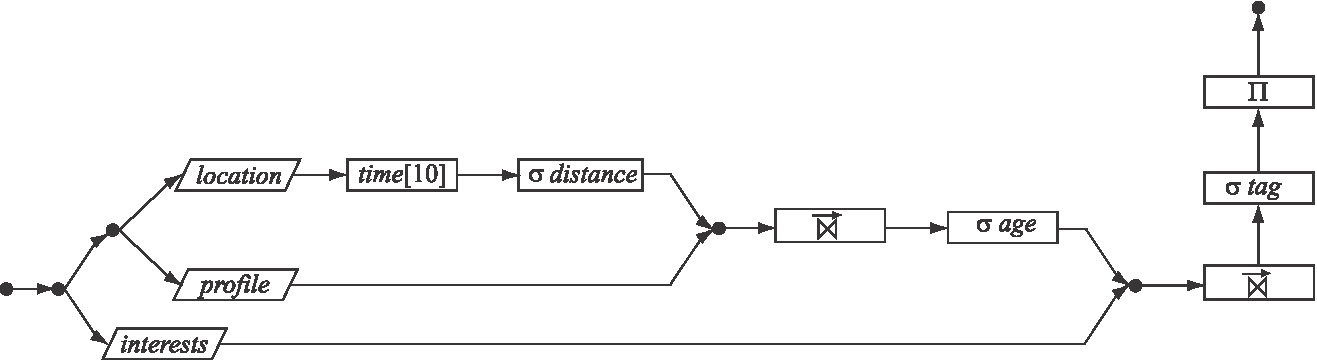
\includegraphics[natwidth=22.26 cm,natheight=6.07cm]{Images/FriendFinderQueryWF.pdf}}
	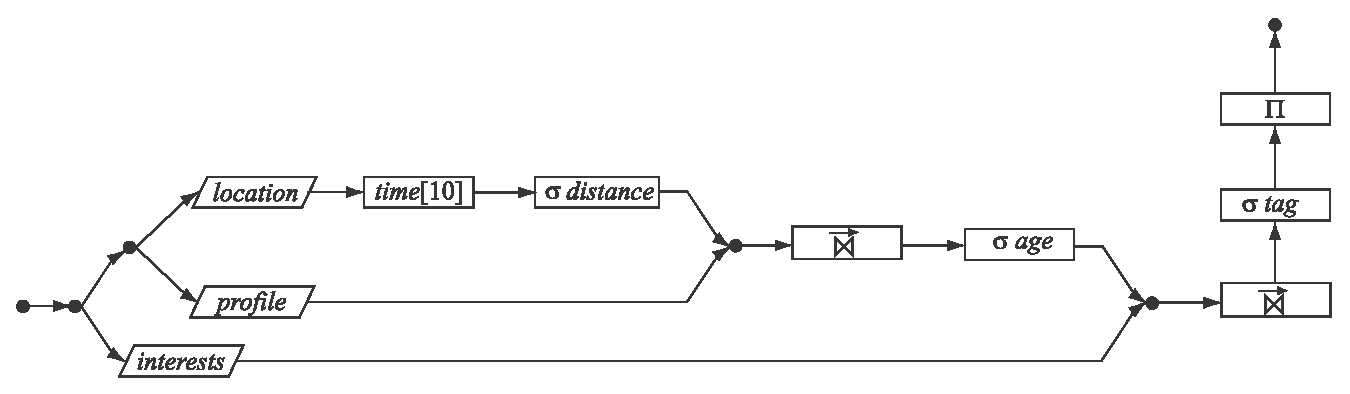
\epsfig{file=Images/FriendFinderQueryWF.eps,scale=0.5}
	\caption{Data-centric workflow for example application}
	\label{fig:servCoorExample}
\end{figure}

A workflow $W$ is modeled as a directed acyclic graph $W=(V, E, in, out, A, C)$ where:
		\begin{center}
			\footnotesize
			\begin{tabular}{rp{7.5cm}}
				$V$                      & is a set of vertices \\
				$E \subseteq V \times V$ & is a set of edges \\
				$A \subseteq V$          & is a set of activities \\
				$\{in, out\} \subseteq A$     & are the initial and final activities of $W$\\
				$C \subseteq V$          & is a set of composition operators $\{par_1,...,par_n\}$\\.     
			\end{tabular}   
		\end{center}
There are three types of vertices: \textit{activities} perform a service method invocation and always have ancestor and descendant vertices, \textit{in} vertices have no ancestors and their only goal is to launch the first \textit{activity} of the workflow, \textit{out} vertices have no descendants and stop the workflow execution after the last \textit{activity}. A series of construction rules enable to generate a workflow graph from a given ASM, which are detailed in \cite{vcv}.

\subsection{Computation services}\label{subsec:computationServices}

Two kinds of computation services form part of our approach: simple computation services and composite computation services specified in the ASASEL language.

%\begin{figure*}
%   \begin{center}
%      \scalebox{0.785}{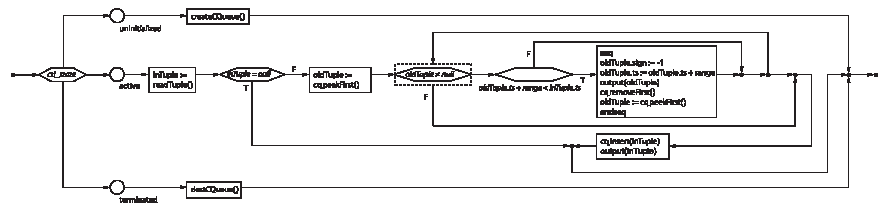
\includegraphics[natwidth=12.31cm,natheight=7.16cm]{Images/time-based-window.pdf}}
%   \end{center}
%   \caption{Workflow representation of the time-based window}
%   \label{fig:timeBasedWindowWF}
%\end{figure*}

\textbf{Simple computation services}  involve a single service operation invocation to process data. For instance, a distance computation service that relies on a \texttt{geo-distance} service, which provides the capability to calculate the geographical distance between two points, e.g., by Vincenty's formula.

\textbf{Composite computation services}  process data by multiple operation invocations, possibly from different services, and often also by the manipulation of local data. These tasks are organized in a service coordination specified in the ASASEL language and represented as a workflow, following a model in which we add data items as well as conditional and iteration constructs to our basic parallel and sequential composition workflow model illustrated in Figure \ref{fig:servCoorExample}.
		
The specification of a time-based window composite service in ASASEL is presented in Listing \ref{TimeWindowListing}, based on a simple \texttt{calendar-queue} service. It has a corresponding workflow representation as detailed in \cite{vcv}.
		
\lstset{language=AbStM,showstringspaces=false}
\begin{lstlisting}[caption={ASM specification for the time-based window},label=TimeWindowListing]
if( ctl_state = 'active')
  seq
     inTuple := readTuple()
     if(inTuple = nil)
        skip
     else
        seq
           oldTuple := cq.peekFirst()
           iterate(oldTuple != nil)
              if(oldTuple.ts + range < inTuple.ts)
                 seq
                    oldTuple.sign := -1
                    oldTuple.ts := oldTuple.ts + range
                    output(oldTuple)
                    cq.removeFirst()
                    oldTuple := cq.peekFirst()
                 endseq
           pq.enqueue(inTuple)
           output(inTuple)
        endseq
  endseq
\end{lstlisting}







		













\section{Complex Values Data Model}\label{sec:complexValuesDataModel}

Our workflow model is complemented by a data model consisting of complex values and operations to flexibly manipulate them. Due to space restrictions we only specify two representative operators while the full specification and semantics of the model is given in \cite{vcv}. Concretely, we first define complex values and then present a recursive operator and a nesting operator over them.

The set $\mathbf{T}$ of all complex value types over a set $\mathbb{A}$ of type names is defined inductively as follows.

\begin{enumerate}
	\item if $D$ is a domain, then $A:D$ is an atomic type named $A$, where $A \in \mathbb{A}$;
	\item if $\hat{t}$ is a type, then $A:\{\hat{t}\}$ is a set type named $A$;
	\item if $\hat{t}_1, ..., \hat{t}_n$ are types with distinct names, then $A:\langle \hat{t}_1, ..., \hat{t}_n \rangle$ is a tuple type named $A$ and each $\hat{t}_i$ is an attribute type.
\end{enumerate}

\subsection{Recursive complex value operators}

Inspired in the traditional relational operators, they apply to complex values in a recursive manner; meaning that through an expression it is possible to apply the operator to structures nested within a complex value. In particular, we present next the specification of the projection operator.

\vspace*{0.25cm}
\textbf{Projection} Enables to retrieve certain data elements in a complex value instance. Such data elements may be nested and multivalued. The data elements to retrieve are specified in a (possibly recursive) projection expression $\pi_{exp}$, which is applied to the input complex value instance \textit{s}.

\begin{itemize}
	\item \textit{Notation}: $\ \pi_{exp}(s)$
	
	Projection expressions $\pi_{exp}$ are constructed as follows, we use $A$ to represent type names that occur in the complex value instance

	\vspace{0.2cm}
   	\noindent \hspace*{1.5cm} $\pi_{exp}$ \hspace*{0.25cm} $\ \ ::= \ \ \pi \ ( \ list \ ) \ \ $ \\
   	\noindent \hspace*{1.5cm} $list$ \hspace*{0.26cm} $\ \ ::= \ \ term \ \ | \ \ term \ , \ list \ \ $ \\
   	\noindent \hspace*{1.5cm} $term$ \hspace*{0.0cm} $\ \ ::= \ \ A \ \ | \ \ \pi_{exp} \ \ $ \\
	\vspace{0.2cm}
	
	\item \textit{Operation type}:
	$\ \pi:\hat{t} \rightarrow \hat{t'}$, where $\hat{t'}$ is defined below
	
	\item \textit{Semantics}: $\pi_{exp}(s)$ is defined as follows.
	
	First, we define the function $eval(A:v, L)$, where $A:v$ is a tuple complex value of the form
	$A:\langle ...,A':v',... \rangle$ and $L$ an expression term (as defined by the notation third rule above).
	
	\begin{enumerate}
		\item If $L$ is of the form $A'$ then $eval(A:v, L)=A':v'$
		\item If $L$ is of the form $\pi(A', L_1',...,L_n')$ then $eval(A:v, L) = \pi(A', L_1',...,L_n')(A':v')$
	\end{enumerate}

	The value of $\pi_{exp}(s)$ is then given by

	\begin{enumerate}
		\item If $s = A:\langle A_1:v_1,...,A_n:v_n \rangle = A:v$, i.e. $s$ is a tuple complex value, and $\pi_{exp} = \pi(A, L_1,...,L_n)$, then \\
					\hspace{1.5cm}$\pi_{exp}(s) = A:\langle eval(A:v, L_1),...,eval(A:v, L_n) \rangle$ and \\
					\hspace{1.5cm}$\hat{t'}$ is $A:\langle type(eval(A:v, L_1)),...,type(eval(A:v, L_n)) \rangle$
		\item If $s = A:\{ A':v_1,...,A':v_m \}$, i.e. $s$ is a set complex value, and $\pi_{exp} = \pi(A, \pi_{exp'})$ with $\pi_{exp'}$ of the form $\pi(A', L_1',...,L_n')$, then \\
     			\hspace{1.5cm}$\pi_{exp}(s) = A:\{ \pi_{exp'}(A':v_i) | A':v_i \in val(s) \} $ and \\
					\hspace{1.5cm}$\hat{t'}$ is $A:\{type(\pi_{exp'}(A':v_j))\}$ for an arbitrary $A':v_j \in val(s)$
	\end{enumerate}

\end{itemize}

\noindent Consider the following complex value

\vspace*{0.25cm}
\noindent \textit{s = person:$\langle$ sex:`M', nick:`Charles', email:`charles@gmail.com', age:40,}

\hspace*{1.0cm} \textit{interests:$\{$stag:$\langle$ tag:`art', score:6.5 $\rangle$, stag:$\langle$ tag:`sports', score:7.5 $\rangle \} \rangle$}

\vspace*{0.25cm}
\noindent The expression $\pi(person, nick, age, \pi(interests, \pi(stag, score)))(s)$ produces the value

\vspace*{0.25cm}
\noindent \textit{$ \ $person:$\langle$ nick:`Charles', age:40,}\hspace*{0.0cm}\textit{interests:$\{$stag:$\langle$ score:6.5 $\rangle$, stag:$\langle$score:7.5 $\rangle \} \rangle \ $}

\subsection{Nesting and unnesting operations}

These operators take into consideration common values occurring in several tuples, therefore facilitating grouping or ungrouping them (which gives the operators their names). The specification of the group operator is presented next.

\vspace*{0.25cm}
\noindent \textbf{Group}. Intuitively, grouping a set of tuple complex values $R$ over a set of attributes $X$ implies aggregating the tuples that are equal in all attributes except those in $X$ to create a single tuple, which will contain a new set attribute with new tuples containing all of the $X$-values of the aggregated input tuples. This set attribute is given a new name, as are the tuples built from the $X$ attributes that are contained in it; both of which are specified in the group expression.

\begin{itemize}
	\item \textit{Notation}: $\ group_{exp}(R)$

	Group expressions $exp$ are constructed as follows, we use $A$ to represent the type names that occur in the complex value instances,
	and $B$ and $B'$ to represent the new names of the grouped tuples set and its constituent tuples, respectively

	\vspace{0.2cm}
   	\noindent \hspace*{1.5cm} $exp$ \hspace*{0.25cm} $\ \ ::= \ \ group \ ( A,\ B:list \ [B'] \ ) \ \ $ \\
   	\noindent \hspace*{1.5cm} $list$ \hspace*{0.26cm} $\ \ ::= \ \ A \ \ | \ \ A \ , \ list \ \ $
	\vspace{0.2cm}
	
	\item \textit{Operation type}:
	
	$group: \ \{A:\langle \hat{a}_1,...,\hat{a}_m,\hat{b}_1,...,\hat{b}_n \rangle\} \rightarrow 
	\{A:\langle \hat{a}_1,...,\hat{a}_m, B:\{B':\langle \hat{b}_1,...,\hat{b}_n \rangle \} \rangle\}$
	
	\item \textit{Semantics}:
	
	$group_{exp}(R)= \\
	\{ A:\langle A_1:v_1,...,A_m:v_m, B:w \rangle \ | \ ( \\
	\hspace*{0.2cm}\exists t \in R \ | \ \forall_{i|1 \leq i \leq m} \ t.A_i = v_i \wedge w=\\
	\hspace*{0.2cm}\{ B':\langle B_1:u_1,...,B_n:u_n \rangle | A:\langle A_1:v'_1,...,A_m:v'_m, B_1:u_1,...,B_n:u_n \rangle \\
	\hspace*{0.2cm}\{ B':\langle B_1:u_1,...,B_n:u_n \rangle | A:\langle A_1:v'_1,...,A_m:v'_m, B_1:u_1,...,B_n:u_n \rangle \\
	\hspace*{0.2cm}\in R \wedge \forall_{i|1 \leq i \leq m} \ t.A_i = v'_i \} \\
	) \ \}$
	
	where all values $A_i:v_i$ and $A_i:v'_i$ are of type $\hat{a}_i$ and all values $B_i:u_i$ are of type $\hat{b}_i$.

\end{itemize}

Consider the following set of tuple complex values

\vspace*{0.25cm}
	\noindent \hspace*{0.5cm} \textit{$R=\{$ \ person:$\langle$ nickname:`Bob', tag:`sports', score:6.5 $\rangle$}	\\
	\hspace*{1.5cm} \textit{person:$\langle$ nickname:`Bob', tag:`cars', score:8.0 $\rangle$}	\\
	\hspace*{1.5cm} \textit{person:$\langle$ nickname:`Alice', tag:`fashion', score:7.0 $\rangle$}	\\
	\hspace*{1.5cm} \textit{person:$\langle$ nickname:`Alice', tag:`novels', score:8.5 $\rangle$ \ $\}$ }

\vspace*{0.25cm}
The expression $group(person, interests:tag, score[s\_tag])(R)$ thus yields:

\vspace{0.25cm}
	\noindent \hspace*{0.5cm} \textit{$R'=\{$ person:$\langle$ nickname:`Bob',}	\\
	\hspace*{2.3cm} \textit{interests:$\{$s\_tag:$\langle$ tag:`sports', score:6.5 $\rangle$,} \\
	\hspace*{3.9cm} \textit{s\_tag:$\langle$tag:`cars', score:8.0 $\rangle$ $\}$,} \\
	\hspace*{1.7cm} \textit{person:$\langle$ nickname:`Alice',}	\\
	\hspace*{2.3cm} \textit{interests:$\{$s\_tag:$\langle$ tag:`fashion', score:7.0 $\rangle$,} \\
	\hspace*{3.9cm} \textit{s\_tag:$\langle$tag:`novels', score:8.5 $\rangle$ $\} \ \}$}









\lstset{ %
        language=Prolog,                % the language of the code
        basicstyle=\scriptsize,       % the size of the fonts that are used for the code
        %numbers=right,                   % where to put the line-numbers
        %numberstyle=\scriptsize,      % the size of the fonts that are used for the line-numbers
        %stepnumber=1,                   % the step between two line-numbers. If it's 1, each line 
                                % will be numbered
        %numbersep=0.05cm,                  % how far the line-numbers are from the code
        backgroundcolor=\color{white},  % choose the background color. You must add \usepackage{color}
        showspaces=false,               % show spaces adding particular underscores
        showstringspaces=false,         % underline spaces within strings
        showtabs=false,                 % show tabs within strings adding particular underscores
        frame=none,                   % adds a frame around the code
        tabsize=3,                      % sets default tabsize to 2 spaces
        captionpos=b,                   % sets the caption-position to bottom
        breaklines=true,                % sets automatic line breaking
        breakatwhitespace=false,        % sets if automatic breaks should only happen at whitespace
        %title=\lstname,                 % show the filename of files included with \lstinputlisting;
                                   % also try caption instead of title
        escapeinside={\%*}{*)},         % if you want to add a comment within your code
        deletekeywords={not},
        aboveskip=5pt,
        belowskip=-3pt,
        %morekeywords={luents, actions, always, initial, if, inertial, after, inertial, noConcurrency,goal,not,caused,executable,nonexecutable,forbiden,requires}            % if you want to add more keywords to the set
}

\section{Workflow enumeration} \label{sec:workflowTransformation}

This section decribes the process of enumerating all the equivalent workflows that satisfy the same functional requirements given by an ASASEL specification. The enumeration leads to a search space of workflows with increasing levels of parallelism in their structure. The levels of parallelism can privilege the cost preferences such as response time or the communication cost. The enumeration is subject to constraints for composing the required activities by the ASASEL specification. We model these constraints as action rules in the language DLV-K\footnote{http://www.dbai.tuwien.ac.at/proj/dlv/k}.

In DLV-K, planning problems have a set of facts that represent the problem domain named background knowledge. The facts are predicates of static knowledge and are the input of the planning problem. Planning problems are modeled as state machines described by a set of fluents and a set of actions. A fluent is a property of an object in the world and is part of the states of the world. Fluents may be true, false or unknown. An action is executable if a precondition holds in the current state. Once an action is executed, the fluents and thus the state of the plan are modified. The action rules define the subset of fluents that must be held before the execution of an action (\ie{} pre-conditions) and the subset of fluents to be held after the execution (\ie{} post-conditions). Finally, a goal is a set of fluents that must be reached at the end of the plan. A goal is expressed by the conjunction of fluents and by a plan length $l \in \mathds{Z}^{+}$.

The mapping from workflow enumeration to a planning problem is shown in Table \ref{tab:mappingQW-PP}. The APIs and the required activities by the ASASEL specification are modeled as facts of the background knowledge. The execution state of a workflow is modeled as fluents and the activities to perform as actions.
	
	\begin{table}
	   \begin{center}
	      \begin{tabular}{|r|l|}
	         \hline
	         \multicolumn{1}{|c|}{\textbf{Workflow }}& \multicolumn{1}{c|}{\textbf{Planning problem}} \\
	         \hline
	         APIs, required activities & Facts (background knowledge) \\
	         \hline
	         Workflow states & Fluents \\
	         \hline
	         Workflow activities & Actions \\
	         \hline
	         Result delivery & Goal: \texttt{finished?(}$l \in \mathds{Z}^{+}$\texttt{)} \\
	         \hline
	      \end{tabular}
	   \end{center} 
	   \caption{Mapping to a planning problem}
	   \label{tab:mappingQW-PP}
	\end{table}
	
Next we show, through an example, how we represent the background knowledge for workflow enumeration. Afterwards, we show how the workflow state and activities are expressed in DLV-K rules. Given such rules, the DLV-K engine performs the workflow enumeration.

\subsection{Background knowledge} \label{subsec:kb}
The background knowledge contains a set of facts that serve as the input for the workflow enumeration. It includes (1) the service methods and (2) the required activities derived from the ASASEL specification.

\vspace*{0.25cm}
\noindent               
\textbf{Service methods} are represented by the facts \texttt{method/2}. The bound and free attributes associated to such a method are represented by the facts \texttt{bound_p/4} and \texttt{free_p/4}. The rule \texttt{att/4} represents the normal form of an attribute.

%\lstinputlisting[lastline=15, fontadjust=true, label=list:service-interfaces,caption={Service interfaces}]{code/service-interfaces-FF.kb}

\lstinputlisting[fontadjust=true, label=list:service-interfaces]{code/service-interfaces-FF.kb}
\vspace*{0.25cm}
\textbf{Required activities} are derived from the ASASEL workflow specification and represented through facts (with the underscore at the end). The required activities derived from a workflow implementing ``\textit{What are the interests of my friend Joe}'' are represented by the following facts. 

%\lstinputlisting[fontadjust=true, label=list:hybridQuery, caption={Hybrid query in facts}]{code/query-FF1.kb}

\lstinputlisting[fontadjust=true, label=list:hybridQuery]{code/query-FF1.kb}
\vspace*{0.25cm}
These required activities express the need over the methods \texttt{p:profl} and \texttt{i:interests}. Both data are retrieved by \texttt{retrieve\_/3} and represented by \texttt{p1} and \texttt{i1}. The nickname attribute of the profile is filtered by \texttt{filter\_/2} and correlated by \texttt{join\_/4} interests through the nickname attribute. The attributes nickname, score and tag are projected. Observe that the filter over the nickname attribute is only indicated as the equality operators are not relevant for the workflow transformation.

\subsection{Workflow activities}
Workflow activities are represented as actions in DLV-K. Such actions are predicates that require facts from the background knowledge to be true. There are also activities that are independent from facts.

\vspace*{0.25cm}
\noindent         
\textbf{init and finish} These activities have the special purpose to initialize and terminate the workflow execution. Thus their semantics is not associated with the application and there is no dependency with the background knowledge.

\vspace*{0.25cm}
\noindent\textbf{data\_service} establishes a connection with a data service method. It requires from the knowledge base a service method and the expressed need to retrieve data from it.

%\lstinputlisting[firstline=23, lastline=23, fontadjust=false, label=list:qw-on-demand, caption={on-demand activity}]{code/aesop.plan}

\lstinputlisting[firstline=23, lastline=24, fontadjust=false, label=list:qw-on-demand]{code/aesop2.plan}
\vspace*{0.25cm}
\textbf{bind\_selection} invokes a service method and retrieves data from it. The invocation is done by providing a bound attribute. 

%\lstinputlisting[firstline=26, lastline=27, fontadjust=false, label=list:qw-bind-selection, caption={bind-selection activity}]{code/aesop.plan}

\lstinputlisting[firstline=27, lastline=28, fontadjust=false, label=list:qw-bind-selection]{code/aesop2.plan}
\vspace*{0.25cm}
\textbf{bind_join} correlates data from two service methods w.r.t. an attribute from each one. The attribute from the outer method must be bound. This activity is analogous to \texttt{bind_selection} but it takes the value from another method attribute.
                     
%\lstinputlisting[firstline=30, lastline=35, fontadjust=false, label=list:qw-bind-join, caption={bind-join activity}]{code/aesop.plan}

\lstinputlisting[firstline=31, lastline=35, fontadjust=false, label=list:qw-bind-join]{code/aesop2.plan}
\vspace*{0.25cm}           
\textbf{filter} performs the filtering over an attribute of a required service method.
            
%\lstinputlisting[firstline=39, lastline=42, fontadjust=false, label=list:qw-select, caption={select activity}]{code/aesop.plan}

\lstinputlisting[firstline=39, lastline=42, fontadjust=false, label=list:qw-select]{code/aesop.plan}
\vspace*{0.25cm}                
\textbf{project} projects an attribute of a service method.
                     
%\lstinputlisting[firstline=44, lastline=44, fontadjust=false, label=list:qw-project, caption={project activity}]{code/aesop.plan}

\lstinputlisting[firstline=44, lastline=44, fontadjust=false, label=list:qw-project]{code/aesop.plan}
\vspace*{0.25cm}			   
The semantics of these activities is completed with constraints that define their pre-conditions and post-conditions.
				
\subsection{Workflow constraints} 
The workflow constraints define the pre-conditions and post-conditions associated to the execution of the workflow activities. A condition is a state of knowledge modifiable by the execution of activities. Through the satisfaction of such conditions, the workflows are transformed.
In the following, we present the intuition of these constraints along with their rules in DLV-k.

\vspace*{0.25cm}              
\noindent\textbf{init and finish} The \textbf{init} activity has no previous activity and its pre-condition is that the workflow has not been \texttt{initiated}. As post-condition, it produces the state \texttt{initiated}. The last activity is \texttt{finish} and there is no other activity to be executed afterwards. Its pre-condition is that there is not evidence that the workflow is \texttt{finished} and the result has been \texttt{delivered} (See \texttt{output} activity below for details about \texttt{delivered}). The post-condition of \texttt{finish} is \texttt{finished} and this is the goal to be reached for the workflow transformation.
                            
%\lstinputlisting[firstline=49, lastline=52, fontadjust=false, label=list:init-activity, caption={\texttt{init} and \texttt{finish} activities}]{code/aesop.plan}

\lstinputlisting[firstline=49, lastline=52, fontadjust=false, label=list:init-activity]{code/aesop.plan}
\vspace*{0.25cm}        
\textbf{data\_service} Once initiated the workflow, the data services must be \texttt{connected(DS)}. This fluent is produced by the execution of the \texttt{data\_service(DS)} activity. 

%\lstinputlisting[firstline=55, lastline=56, fontadjust=false, label=list:on-demand-activity, caption={on-demand activity}]{code/aesop.plan}

\lstinputlisting[firstline=55, lastline=56, fontadjust=false, label=list:on-demand-activity]{code/aesop.plan}
\vspace*{0.25cm}
In order to retrieve all the required data, all data services should be connected. The fluent \texttt{all_connected} that is false if there is not evidence that a data service is connected. Otherwise, it is true.

%\lstinputlisting[firstline=58, lastline=59, fontadjust=false, label=list:all-connected-fluent, caption={all\_connected fluent}]{code/aesop.plan}

\lstinputlisting[firstline=58, lastline=59, fontadjust=false, label=list:all-connected-fluent]{code/aesop.plan}
\vspace*{0.25cm}
\textbf{bind_selection} It is only executable if there is not evidence that data from the data service \texttt{DS} have been retrieved and if there is a connection with \texttt{DS}. Once the bind selection is executed, the fluent \texttt{retrieved(DS)} is true. 

      
%\lstinputlisting[firstline=61, lastline=63, fontadjust=false, label=list:bind-selection-activity, caption={bind\_ selection activity}]{code/aesop.plan}

\lstinputlisting[firstline=61, lastline=63, fontadjust=false, label=list:bind-selection-activity]{code/aesop.plan}
\vspace*{0.25cm}
\textbf{filter} It is executable if there is not evidence that the attribute \texttt{P} of \texttt{DS} has been filtered. It is required that the data from \texttt{DS} have been retrieved and the activity \texttt{select_(DS,P)} must be required. The execution of the filter makes the fluent \texttt{filtered(DS,P)} true.

%\lstinputlisting[firstline=74, lastline=76, fontadjust=false, label=list:select-activity, caption={select activity}]{code/aesop.plan}

\lstinputlisting[firstline=74, lastline=76, fontadjust=false, label=list:select-activity]{code/aesop2.plan}
\vspace*{0.25cm}
As might several filter activities over \texttt{DS} are required, the \texttt{all_filtered_from} becomes true if there is no other attribute pending to be filtered.

%\lstinputlisting[firstline=77, lastline=78, fontadjust=false, label=list:all-selected-from, caption={all\_select\_from fluent}]{code/aesop.plan}

\lstinputlisting[firstline=77, lastline=80, fontadjust=false, label=list:all-selected-from]{code/aesop2.plan}
\vspace*{0.25cm}
There is the fluent \texttt{all\_filtered} that becomes true if there is no other attribute of the method \texttt{DS} pending to be filtered.

%\lstinputlisting[firstline=80, lastline=82, fontadjust=false, label=list:all-selected, caption={all\_select fluent}]{code/aesop.plan}

\lstinputlisting[firstline=80, lastline=82, fontadjust=false, label=list:all-selected]{code/aesop.plan}
\vspace*{0.25cm}
\textbf{project} This activity is executable if there is not evidence that the attribute \texttt{P} of \texttt{DS} has been projected. The execution of projection makes the fluent \texttt{projected} true.
               
%\lstinputlisting[firstline=84, lastline=85, fontadjust=false, label=list:project, caption={project activity}]{code/aesop.plan}

\lstinputlisting[firstline=84, lastline=85, fontadjust=false, label=list:project]{code/aesop.plan}
\vspace*{0.25cm}
During the workflow execution, all the projection activities have to  be performed. For the method \texttt{DS}, the fluent \texttt{all\_projected\_from} is true if there is no other attribute from \texttt{DS} pending to be projected. The fluent \texttt{all\_projected} is true if there is no other \texttt{DS} with an attribute pending to be projected.
                
%\lstinputlisting[firstline=88, lastline=92, fontadjust=false, label=list:all-projected-from, caption={all\_projected\_from fluent}]{code/aesop.plan}

\lstinputlisting[firstline=88, lastline=94, fontadjust=false, label=list:all-projected-from]{code/aesop.plan}
\vspace*{0.25cm}                  
\textbf{output} Once all the required activities are performed, the result is delivered by the activity \texttt{output}. To model this pre-condition, the fluent \texttt{activities\_performed} is true if all the required activities have been processed. Otherwise, the fluent is false \texttt{-activities\_performed}.

%\lstinputlisting[firstline=95, lastline=99, fontadjust=false, label=list:query-processed, caption={query\_processed fluent}]{code/aesop.plan}

\lstinputlisting[firstline=95, lastline=99, fontadjust=false, label=list:query-processed]{code/aesop.plan}
\vspace*{0.25cm}
Once the result is delivered by \texttt{output}, the fluent \texttt{delivered} becomes true and the workflow can be finished (\cf{} \texttt{finish} pre-conditions).

%\lstinputlisting[firstline=101, lastline=102, fontadjust=false, label=list:output, caption={output fluent}]{code/aesop.plan}

\lstinputlisting[firstline=101, lastline=103, fontadjust=false, label=list:output]{code/aesop.plan}







\section{Experiments} \label{sec:experiments}
\def\maxpar{\textit{par$^{+}$}}
\def\parminus{\textit{seq$^{+}$}}

We performed experiments to measure the amount of alternative workflows with sequential compositions and with parallel compositions for a given ASASEL workflow.
We setup seven different ASASEL workflows $WF^{1},...,WF^{7}$ with increasing number of activities and different potential grades of parallelism.
The generated workflows were classified by analyzing the data dependencies among activities and their structures.
A workflow whose independent activities are composed in parallel is classified as \maxpar{}, otherwise it is classified as \parminus{}.
The charts in Figure \ref{fig:impl:ssDFCF} show the search spaces with the classification of workflows and the required time for each ASASEL workflow $WF^{1},...,WF^{7}$.


	\begin{figure}
		\centering
		\begin{tabular}{lr}
				\subfloat[Clasification of the search spaces]{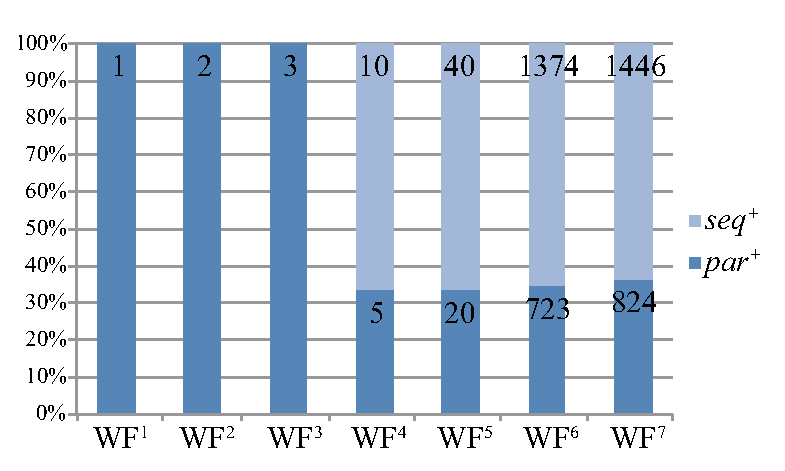
\epsfig{file=Images/ssClassification.eps,scale=0.5}	\label{fig:searchspaceClassification}}
				&
				\subfloat[Required time]{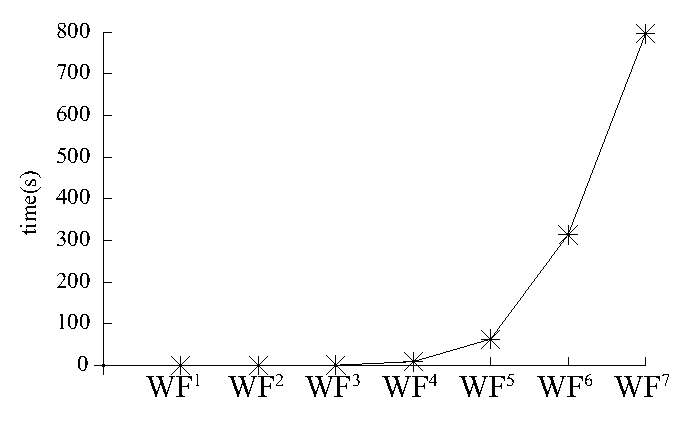
\epsfig{file=Images/time.eps, scale=0.5}\label{fig:timeGraph}}			
		\end{tabular}
		\caption{Enumeration of the space of alternative workflows with different grade of parallelism}
		\label{fig:impl:ssDFCF}
	\end{figure}
				
In Figure \ref{fig:searchspaceClassification}, the search spaces of the workflows $WF^{1}-WF^{3}$ only contain \maxpar{} workflows because they have few activities and there are no independent activities.
The search spaces of the workflows $WF^{4}-WF^{7}$ have ~1/3 of \maxpar{} workflows and ~2/3 \parminus{} workflows. 
This correspondence is not constant and depends on the data dependencies among activities, \eg{} a workflow with many activities may have only sequential alternatives if there are no independent activities.

The \maxpar{} workflows represent better opportunities for improving time related costs while the \parminus{} ones privilege the resource usage (\eg{} network, cpu).
This classification can be used for improving the enumeration performance (\cf{} Figure \ref{fig:timeGraph}) by incorporating user/application preferences for obtaining only \maxpar{} or \parminus{}.

 
%%\vspace*{1cm}
%%
%%
%%We defined four workflow cases with different number of required activities based on the example of Section \ref{subsec:kb}. We performed experiments for measuring the size of the search space given the expected length of workflows. The length determines the size of the search space and thus the required time to perform the transformation. We used lengths from 6 to 14.
%%
%%The growth of the search space is shown in Figure \ref{fig:graphs}. The size tends to be stable once it has reached the maximum length with all the required activities composed in sequence. For instance, $W1$ has $11$ required activities and it reaches the maximum length with $l=11$. The workflows with the "maximum" number of parallel compositions are the ones with the small $l$. For instance with $l=7$, $W1$ has the maximum number of parallel compositions\footnote{See http://goo.gl/XKZuL and http://goo.gl/z4iu3 for examples of lengths 7 and 11.}.
%%
%%%\tabsize{tab:size}{Search space growth respect to the plan length}
%%
%%%\tabtime{tab:time}{Time for workflow transformations with different lengths}
%%
%%\begin{figure*}
%%	\centering
%%		\begin{tabular}{lr}
%%%				\subfloat[Search space]{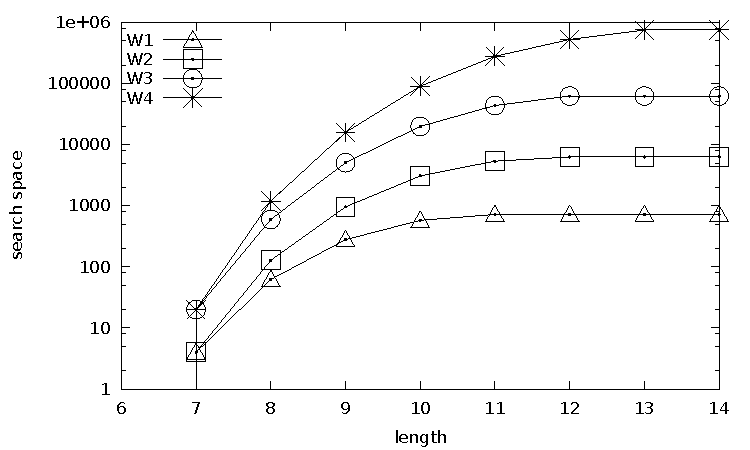
\epsfig{file=Images/searchspace.pdf, scale=0.47}\label{fig:searchspaceGraph}}
%%				&
%%%				\subfloat[Execution time]{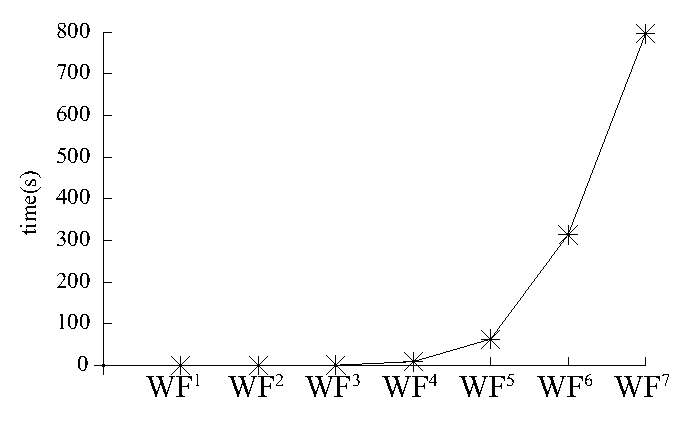
\epsfig{file=Images/time.eps, scale=0.47}\label{fig:timeGraph}}			
%%		\end{tabular}
%%		\caption{Search space and execution time}
%%		\label{fig:graphs}
%%\end{figure*}
%%
%%Besides the size of search space, the time for processing the workflow generation is exponential (\cf{} Figure \ref{fig:graphs}) and it is not feasible to generate completely the search space. Future work involves exploring alternative encodings and planning systems to obtain better performance.




\section{System Implementation} \label{sec:asasel:demo}
	
The ASASEL system was developed on the Java platform. Workflows are entered textually via a GUI illustrated in Figure \ref{fig:asaselGUI}. For a given ASASEL service coordination, the GUI (relying on the JGraph\footnote{http://www.jgraph.com/} library) provides the user a workflow visualization. Data services are represented in yellow whereas computation services are represented in blue, both with their corresponding labels.

The enactment of a workflow is enabled by two main components. First, a scheduler determines which service is executed at a given time according to a predefined policy. Second, composite services are executed by an interpreter that implements the full ASASEL language. Computation service workflows can also be visualized through the GUI, as shown at the right part of the screenshot in Figure \ref{fig:asaselGUI}. The interpreter was developed using the ANTLR\footnote{http://www.antlr.org/} parser generator.
	
During the execution of a workflow, data flows from the data services to several computation services via queues, as determined by the ASASEL specification. Computation services can be specified to output data in textual form in the GUI or to transmit it to another application. For instance, in our example application we output as a result data stream that denotes the tuples that are added and the tuples that are removed from the result dataset.
	
We developed a set of basic computation services that are used to build the operations for our example application. These services run on a Tomcat container supported by the JAX-WS reference implementation \footnote{https://jax-ws.dev.java.net/}, which enables to create stateful services.
	
Additionally, we implemented two test scenarios and their corresponding data services to use with our computation services. The first one is the location-based application introduced in Section \ref{sec:serviceOrientedWorkflows}. The second scenario is an adaptation of the online auctions NEXMark benchmark\footnote{http://datalab.cs.pdx.edu/niagara/NEXMark/} for XML stream query processing which we employed to obtain performance measurements. In brief, the measurements indicated a tolerable overhead for the use of services, which we consider outweighed by the advantages.
	
	%\begin{figure*}
	%	\centering
	%	\epsfig{file=Images/ASASEL.eps, scale=0.37}
	%	\caption{}
	%	\label{fig:asaselGUI}
	%\end{figure*}
	
	\begin{figure}
   \begin{center}
     \scalebox{0.675}{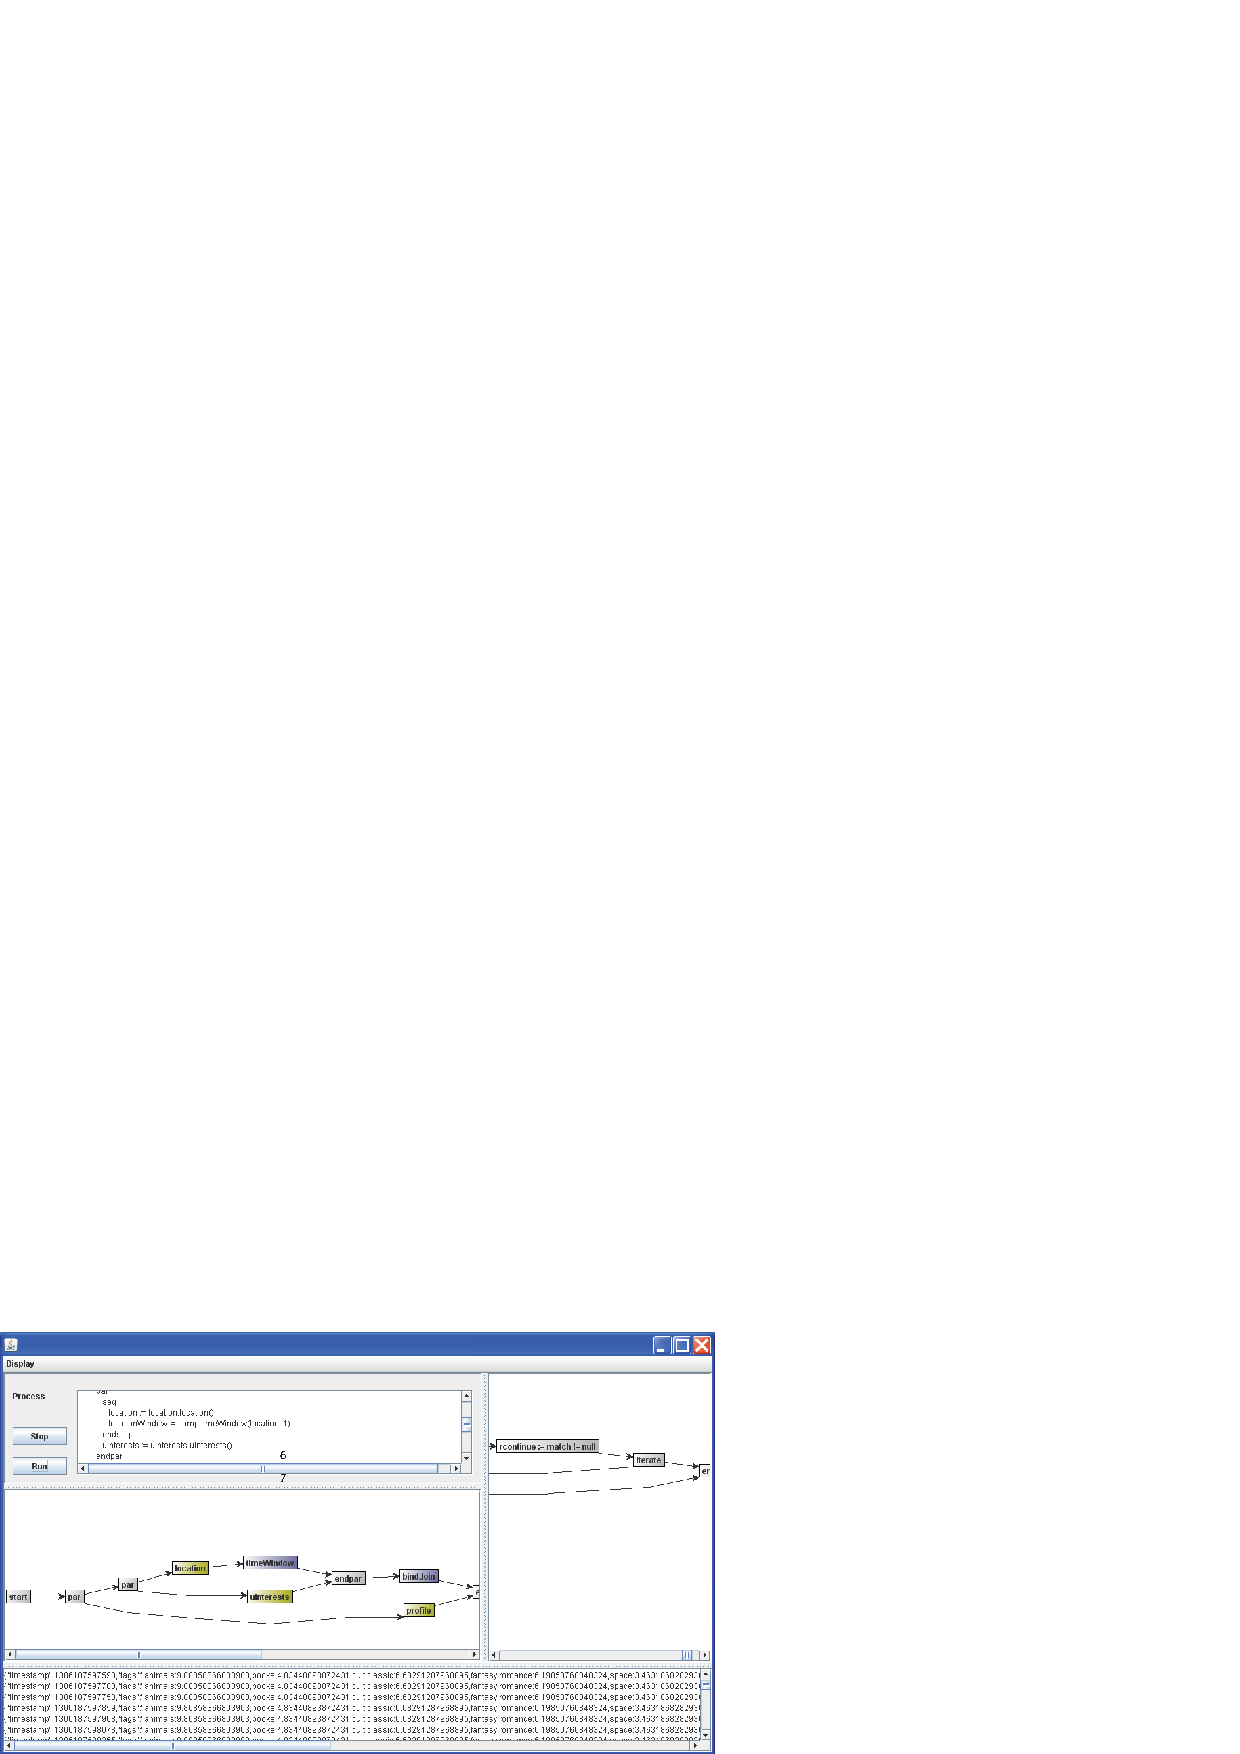
\includegraphics[natwidth=12.31cm,natheight=7.16cm]{Images/asaselgui.pdf}}
   \end{center}
   \caption{Caption of the ASASEL GUI}
   \label{fig:asaselGUI}
\end{figure}




\section{Related work} \label{sec:relatedwork}

At their top level, service-oriented workflows involving data operations share some similarities with queries over Web services as presented in \cite{Srivastava:2006:QOO:1182635.1164159}. There the authors propose an optimization approach by ordering the service calls in a pipelined fashion and by tuning the size of service call batches. An algebraic approach for the optimization of workflows with relational and map-reduce operations is presented in \cite{DBLP:journals/pvldb/OgasawaraOVDPM11}. Our approach is to enable workflows with a broader variety of operations defined through service compositions, thus requiring alternative optimization techniques.

Alternative formalisms for the specification of workflows include, for example, process algebras \cite{Curcin:2011:STW:2048456.2048467} and petri nets \cite{Hidders:2008:DDL:1340791.1340907}. Although ASMs have been used to study and model the properties of workflows, less effort has been given to using them in a fully operational manner. The combination of data-flow and control-flow present in our approach has some similarities with the work presented in \cite{Bowers:2006:ESR:1129755.1130113}. However, they focus on complementing a workflow model with control-flow structures for tasks such as fault-tolerant and adaptive distributed data transfer, whereas we focus on enabling the composition of services to support new functionality.




\section{Conclusions and future work} \label{sec:conclusions}

In this paper we presented a language and system for the specification and enactment of data-centric workflows based on service composition. In addition, we introduced a planning-based approach for the generation of the search space of workflow transformations. Concretely, we proposed a set of constraints modeled in an action language, specifically DLV-K, in order to characterize the transformation of workflows with sequential and parallel compositions. This work is envisaged to be a foundation for incorporating a full cost model that covers the specification of composite computation services, leading to the selection of the most suitable workflow w.r.t. the user's preferences. Future work involves incorporating the cost model, while also exploring alternative encodings and planning systems to obtain better performance.



%}
%	In this paper we presented the constraints for generating query workflows that model the plans of hybrid queries.
%	The constraints represent the semantics of query workflow activities that is that implement data operators for evaluating a hybrid query.
%	We used the action language DLV-K for modeling the planing problem of query workflow generation in order to get a first (and naive) search space generation towards the optimization of hybrid queries.
%	The results show that time complexity for query workflow generation is exponential. 
%      
%	The constraints must be extended in order to consider the continuous data operators for completely modeling hybrid queries.
%	These constraints can be taken to model a more sophisticated query workflow generation.
%	This implies the abstraction of data operators types and their associated constraints in a general form. 
%
%	Theoretically, query workflow generation can be modeled mathematically by taking the constraints presented here and modeling an objective function.
%	Additionally, the equivalence and coherence of query workflows must be proved.


	
%
% ---- Bibliography ----
%
%\bibliographystyle{alpha}
\bibliographystyle{splncs03}
\bibliography{library/library}

\end{document}
